%+----------------------------------------------------------------------------+
%| SLIDES: Longer presentation on my paper 1805.01696
%| Chapter: Backup slides
%| Author: Antonio miti
%| Event: Visit in Salerno, March 2019
%+----------------------------------------------------------------------------+

%- HandOut Flag -----------------------------------------------------------------------------------------
\newif\ifHandout
	\Handouttrue  %uncomment for the printable version

%- D0cum3nt ----------------------------------------------------------------------------------------------
\documentclass[beamer,10pt]{standalone}



%- Packages ----------------------------------------------------------------------------------------------
\usepackage{verbatim}
\usepackage{appendixnumberbeamer}

\usepackage{amsmath, amssymb}
\usepackage{tikz}

\usepackage{tikz-cd}
\usepackage{graphicx, animate}
\usepackage{hyperref}
\usepackage[english]{babel}
\usepackage{csquotes}
\usepackage[mode=buildnew,subpreambles=true]{standalone}
\usepackage{stackengine}


\providecommand{\blank}{\text{\textvisiblespace}}

%--Beamer Style-----------------------------------------------------------------------------------------------
\usetheme{toninus}

%--WORKAROUND------------------------------------------------------------------------------------------
%Credit: https://tex.stackexchange.com/questions/147899/path-problem-with-included-file-inside-of-a-standalone-file
\providecommand{\includestandalonewithpath}[3][]{%
  \begingroup%
  \providecommand{\datapath}{#2}%
  \includestandalone[#1]{\datapath/#3}%
  \endgroup}




%---------------------------------------------------------------------------------------------------------------------------------------------------
%- D0cum3nt ----------------------------------------------------------------------------------------------------------------------------------
\begin{document}
%------------------------------------------------------------------------------------------------

%------------------------------------------------------------------------------------------------
\begin{frame}
	\begin{center}
	\Huge\emph{EXTRA}
	\end{center}
\end{frame}
\addtocounter{framenumber}{-1}


 %------------------------------------------------------------------------------------------------
  \begin{frame}[fragile,t]{Chevalley-Eilenberg Complex}\label{frame:CE-complex}
  	Consider $\mathfrak{g}$, Lie Algebra.
  	\begin{defblock}[Eilenberg-Chevalley Complex]
  		Chain Complex
			\begin{center}
				\begin{tikzcd}[column sep= small,row sep=0.25ex]
					\ldots \ar[r,"\partial"] & \wedge^k \mathfrak{g} \ar[r,"\partial"] & 
					\wedge^{k-1} \mathfrak{g} \ar[r,"\partial"] & \ldots
			\end{tikzcd}	
			\end{center}
			with chain group
			\begin{displaymath}
				C^k := \wedge^k \mathfrak{g} \equiv 
				\big\{ c : \mathfrak{g}^\ast\times\ldots\mathfrak{g}^\ast \to \mathbb{R}\:\big\vert\, \textrm{alternating, k-linear} \big\}
			\end{displaymath}
			and boundary operator defined as
			$\partial \equiv \partial^k :  \Lambda^{k} {\mathfrak g} \to \Lambda^{k-1} {\mathfrak g}$  via
			$$
				\partial (\xi_1 \wedge \xi_2 \wedge \dots \wedge \xi_k) := \sum_{1\leq i< j \leq k} (-1)^{i+j}\, [\xi_i, \xi_j] \wedge \xi_1 \wedge \dots {\hat \xi}_i \wedge \dots \wedge {\hat \xi}_j \wedge \dots \xi_k
			$$
			where $\hat{}$ denoting deletion and with $\partial_0 = 0$.
  	\end{defblock}
		\begin{claimblock}
			$$\partial^2 = 0$$
		\end{claimblock}		
  \end{frame}
  \note{}
%------------------------------------------------------------------------------------------------

%------------------------------------------------------------------------------------------------
  \begin{frame}[shrink]{Riemannian Generalization}\label{frame:RiemannianGeneralization}
			\begin{columns}
				\begin{column}{.5\linewidth}
					\begin{itemize}
						\item  $(M,g)$ be a connected compact oriented Riemannian manifold of dimension $n+1$
						\item such that the {\it de Rham} cohomology groups $H_{dR}^{k}(M)$ vanish for $k=1,2,\dots n-1$ 
						\item endow it with the multisymplectic form $\nu$ given by its Riemannian volume form
						\item consider $g_0$, lie algebra consisting of divergence-free vector fields vanishing at a point $x_0 \in M$.
					\end{itemize}
					\begin{claimblock}
						$\exists (f)$, family of HCMM, pertaining to the infinitesimal action of $\mathfrak{g}_0$ on $M$
					\end{claimblock}
				\end{column}
				\begin{column}{.5\linewidth}
 			 		\includestandalone[width=\textwidth]{Pictures/Figure_Riemann_Trigger}
				\end{column}
			\end{columns}
		\textit{Sketch of proof:}\\
			The defining formula triggers a recursive construction starting from $f_1$.\\
			Take $ f_1(\xi) := -\Delta^{-1} \delta (\iota_{\xi} \nu)$
			$\quad$ (...) (see \cite{Miti2018})
  \end{frame}
  		\note[itemize]{
			%\item[(Thm)] A hydrodynamically flavoured HCMM can be similarly construed also for an $(n+1)$-dimensional connected, compact, orientable Riemannian manifold $(M,g)$, upon taking its Riemannian volume form $\nu$ as a multisymplectic form and again the group $G$ of volume preserving diffeomorphism group as symmetry group.
			\item[(recall)] The divergence of a vector field $X$ is defined via ${\rm div}\, X := *d\!*\!X^{\flat} = -\delta X^{\flat} $.
			\item The recursive construction start from $f_1$, up to topological obstructions  since we have a sequence of closed forms, which must be actually exact, together with the constraint $ f_n(\partial q) = (-1)^{\frac{(n+1)(n+2)}{2}}\nu(\xi_1,\dots\xi_{n+1})$, with $q= \xi_1 \wedge \dots \xi_{n+1}$, for the {\it constant} function $\mu_{n+1}(\cdot)$.
				\item A natural candidate for the (n-1)-form $f_1$ can be manufactured via Hodge theory as 
				$f_1(\xi) := -\Delta^{-1} \delta (\iota_{\xi} \nu)$
			after imposing $\delta f_1({\xi}) = 0$ (the analogue of the Coulomb gauge condition).
			\item Condition $H_{dR}^{n-1}(M) = 0$ assure one can safely invert the Hodge Laplacian $\Delta = d\delta + \delta d$;
			\item The 	topological assumptions made ensure that the entire procedure goes through unimpeded due to the formula
			$$
			df_k (\xi_1 \wedge\dots \wedge \xi_k) = \mu_k (\xi_1 \wedge\dots \wedge \xi_k), \qquad \qquad k=2,3,\dots n
			$$
			\item Finally, one has to check that 
			$$
			f_n (\partial (\xi_1 \wedge\dots \wedge \xi_{n+1})) =  -\varsigma(n+1) \iota (\xi_1 \wedge\dots \wedge \xi_{n+1})\nu
			$$
			this is guaranteed by the vanishing of all fields at $x_0$.
			% this is true once we notice that, since $c_{x_0} = 0$, the class $[c_x] = 0$ ( see \cite{Callies2016}, section 9).\qed
		}
%------------------------------------------------------------------------------------------------  

%------------------------------------------------------------------------------------------------
  \begin{frame}[fragile]{Loop spaces and transgression}\label{frame:LoopSpacesTransgression}
		\begin{columns}
			%
			\begin{column}[T]{0.5\textwidth}
				Consider any manifold $M$
				\begin{defblock}[Free loop space $LM$(Brilinsky)]
					$$ LM = C^\infty(S^{1},M)	$$
				\end{defblock}
			\end{column}
			%
			\begin{column}[T]{0.5\textwidth}		
				\begin{propblock}[$LM$ is an $\infty$-dimensional Fr\'echet manifold]		
					See \cite{Brylinski1993}.
				\end{propblock}
			\end{column}
			%
		\end{columns}
		
		\begin{defblock}[Tangent space at $\gamma \in LM$]
			\begin{displaymath}
				T_{\gamma}LM = C^\infty(S^{1},\gamma^{\ast}TM)= \Gamma^\infty(\gamma^\ast TM)	
			\end{displaymath}
		\end{defblock}

		\begin{defblock}[Trasgression]
			\begin{columns}
				%
				\begin{column}[t]{0.35\textwidth}
					\centering
					Degree $-1$ chain map
				\end{column}
				%
				\begin{column}{0.65\textwidth}
					\[
						\begin{tikzcd}[column sep= small,row sep=0ex]
					    \ell \colon& \Omega^{\bullet}(M) 	\arrow[r]& \Omega^{\bullet -1}(LM) \\
			  		  & \alpha (\textvisiblespace)\arrow[r, mapsto]& 	\left.\alpha^{\ell} \right\vert_{\gamma} =
			    		\left.{\displaystyle\int^{2\pi}_{0} \iota_{\dot{\gamma}}\alpha(\textvisiblespace)} \right\vert_{\gamma(s)} ~ ds
						\end{tikzcd}	
					\]
				\end{column}
				%
			\end{columns}
		\end{defblock}

		\begin{propblock}[Any pre-$n$-plectic structure $\omega$ on $M$ gives a pre-$(n-1)$-plectic structure $\omega^{\ell}$ on $LM$]
		Transgression commutes with the de Rham differential.
		\end{propblock}

  \end{frame}
	\note{
		a
	}  

%------------------------------------------------------------------------------------------------  

%------------------------------------------------------------------------------------------------
\begin{frame}[fragile]{Transgression and HCMM}\label{frame:TransgressionHCMM}
  	\begin{propblock}[$G$-action on $M$ induces action on $LM$]
  		Given $G$-action $G \times M \to M$, we define a ``point-wise''  action $G \times LM \to LM$ given by:
		\[
			(g \cdot \gamma)(s) = g \cdot\gamma(s) \quad \forall g \in G, ~
			\forall \gamma \in LM
		\]
  	\end{propblock}
		
		\begin{propblock}[HCMM for $G\circlearrowright (M,\omega)$ trasgress to a HCMM for  $G\circlearrowright\left(C^\infty(\Sigma,M), \omega^\ell\right)$]
			If $(M,\omega)$ is a pre-2-plectic manifold equipped with a
			$G$-action and a homotopy moment map
			$f \colon \mathfrak{g} \to L_{\infty}(M,\omega)$, then
		 \begin{align*}
			 \psi : \mathfrak{g} & \to C^\infty(LM)\\
    	 x & \mapsto (f_1(x))^{\ell}
  	\end{align*} is a  moment map for
the induced action of $G$ on the pre-symplectic loop space $(LM,\omega^{\ell})$
		\end{propblock}
\end{frame}
	\note{
		\textbf{Intro by\cite{Callies2016}}\\
		\begin{displayquote}
			Homotopy moment maps for $G$-actions on pre-$2$-plectic manifolds $(M,\omega)$ can be transgressed to ordinary moment maps on the associated pre-symplectic loop space $LM$.

			Motivation for studying such actions arises, for example, in topological field theory. There one can consider a group of symmetries $G$ acting on a ``target space'' $M$ equipped with a closed form $\omega$.\\
The form can be transgressed to a mapping space $\mathrm{Map}(X,M)$ i.e.\ the ``space of fields''.\\ 

			Roughly speaking, this demonstrates how the higher symplectic geometry on $M$ can interact with the ordinary geometry on $\mathrm{Map}(X,M)$.		
		\end{displayquote}
	}  
%------------------------------------------------------------------------------------------------


%------------------------------------------------------------------------------------------------
  \begin{frame}{Rasetti Regge currents} \label{frame:RRcurrents}
  		Dynamics of a perfect fluid (incompressible and inviscid) localized in an open subset $\Omega$ 
  		of $(M,g)$ Riemannian manifold is ruled by the \emph{Euler equations}
  		\begin{columns}
				\begin{column}[T]{0.5\textwidth}
  					\begin{displaymath}\tag{EE}
							\begin{cases}
								\frac{\partial u}{\partial t} + \nabla_u u & = -\nabla p  \\
								\textrm{div} u &= 0 \qquad \textrm{in } \Omega \\
								u \cdot \hat{n} &= 0 \qquad \textrm{on } \partial \Omega \\
							\end{cases}
			  		\end{displaymath}
		  		($u$ is the velocity field of the fluid)
				\end{column}
				\vline
				\begin{column}[T]{0.5\textwidth}
  					\begin{displaymath}\tag{EE vorticity form}
							\begin{cases}
			  				\frac{\partial \omega}{\partial t} &= [\omega, u] \\
								\omega &= \textrm{curl}\left( u \right)  \\
							\end{cases}
			  		\end{displaymath}
				\begin{displaymath}
					[a,b] = \textrm{curl}\left( a \times b \right) \quad \forall a,b \in sdiff(M)		
				\end{displaymath}	
					(Implying that $u$ is divergence free)\\	
				\end{column}
			\end{columns}
			%
			\begin{asideblock}[Rasetti-Regge current are introduced in the context of \alert{vortices theory}]
			\begin{columns}
				\begin{column}{0.85\textwidth}
					Consider a field configuration $v$ with vorticity $\omega= \delta_\gamma$ 
					concentrated on a closed loop $\gamma: S^1 \to \mathbb{R}^3$\\
					Therefore:
					\begin{displaymath}
						\lambda_b(v) := \int v \cdot b = \int v \cdot \textrm{curl}(B) = -\int \omega \cdot B= \oint_\gamma B	
					\end{displaymath}	
					where $B$ is a vector potential of $b$.
				\end{column}
				\begin{column}{0.15\textwidth}
					\vfill
					\includestandalone[width=\textwidth]{Pictures/Figure_vortexloop}	
				\end{column}
			\end{columns}
			\end{asideblock}
			\begin{claimblock}
				EE are equivalent to $\partial_t \lambda_b = \lbrace\lambda_b, H \rbrace$ 
				with $H=\frac{1}{2}\langle v,v\rangle$.				
			\end{claimblock}
  \end{frame}
	\note{
		One this connection between hydrodynamics, vortices and knots see for examples  the notes of Mauro Spera at 
		\href{http://www.math.univ-metz.fr/~wurzbacher/GEMSA.html}{Workshop on multisymplectic geometry and applications    }	
		\\
		Also, notes by Renzo Ricca at
		\href{http://www.matapp.unimib.it/~/ricca/teaching/Ravello1.pdf}{Ravello summer school} and
		\href{http://www.matapp.unimib.it/~/ricca/teaching/Torino3.pdf}{Torino}
				}	

%------------------------------------------------------------------------------------------------


%------------------------------------------------------------------------------------------------
  \begin{frame}[fragile]{GIMMSY construction} \label{frame:Gimmsy}
  		\includestandalone[width=0.90\textwidth]{Pictures/Figure_ms_landscape}  	
  \end{frame}
  \note{}
%------------------------------------------------------------------------------------------------

%------------------------------------------------------------------------------------------------
\begin{frame}[fragile]{$L-\infty$ Algebras (Stasheff, Lada)} 
	\begin{defblock}[$L-\infty$ Algebra]
		\includestandalone[width=0.95\textwidth]{Pictures/Figure_Linfty}	
		\par
		satisfying a \emph{generalized Jacobi identity}
		\begin{displaymath}
			\mathop{\sum_{i+j=k+1}}_{\sigma\in\text{ush}(i,k-i)}
			%\sum_{i+j=k+1}\sum_{\sigma\in\text{ush}(i,k-i)}
			\Big[\text{"sign"} \Big]\,
			\Big[ 	l_j\left(l_i\left(x_{\sigma_1},\ldots,x_{\sigma_i}\right),x_{\sigma_{i+1}},\ldots,x_{\sigma_k}\right)\Big]
			= 0
		\end{displaymath}
		$\forall k\geq 1$ and $x_1,\ldots,x_n \in L$ homogeneus elements.
	\end{defblock}
%	\begin{displaymath}
%		\Big[\text{"sign"} \Big]\, =	(-)^{i(j+1)}\epsilon(\sigma;x_1,\ldots,x_k) \text{sign}(\sigma)
%	\end{displaymath}
	\begin{defblock}[$L-n$ Algebra]
		$L-\infty$ Algebra with $L$ concentred in degrees $(0,\ldots, n-1)$
	\end{defblock}

\end{frame}
\note[itemize]{
  %\item L$\infty$-algebra of observables is a particular instance of a general concept.
  \item L$\infty$-algebras are an higher generalization of differential graded lie algebras
  \item Here we are using a "hands-on" approach to the definition, there are more conceptual presentation of this concept e.g. using co-algebras and coderivation or using operads.
  \item Multi-brackets are:
  \begin{itemize}
		\item (multilinear as a map $l_k: L \times \ldots \times L \rightarrow L$)
		\item graded skewsymmetric
		\item $\textrm{deg}(l_k)=2-k$
		    				\footnote{i.e.$\textrm{deg}\left(l_k(x_1,\ldots,x_k)\right)= \sum_i \textrm{deg}(x_i) +2 -k $}  
  \end{itemize}
  \item (Notation: ) $k\in\mathbb{N}$ I mean the strictly positive natural numbers (i.e $n>0$)
 	\item Unshuffles: 
 		\begin{displaymath}
	    	\begin{split}
				ush(p,q) = \big\lbrace	\sigma \in S_{p+q} \,\big\vert & \, \sigma(i) < \sigma(i+1) \\ 
				& \quad \forall i \neq p \big\rbrace	    		
			\end{split}	    	
	    	\end{displaymath}
	 \item Koszul sign keep track of the sign that comes out when permuting element in odd degree
}
%------------------------------------------------------------------------------------------------

%\includestandalone{Pictures/Frame_PoissonSign}
%\includestandalonewithpath[]{Pictures}{Frame_PoissonSign}




%------------------------------------------------------------------------------------------------
\begin{frame}[fragile,shrink]{Unwrapping the \emph{higher Jacobi identity}} 
\underline{Slogan:} \emph{Jacobi identity satisfied up to an higher coherent homotopy}
%
\begin{table}[]
	\begin{tabular}{ l p{7cm}}
		& $l_1=d$, i.e. there is an underlying chain complex \\
		\begin{tikzcd}
		L \otimes L \ar[r,"d_{\text{tot}}"] \ar[d,"{[\cdot , \cdot]_2}"'] & L \otimes L \ar[d,"{[\cdot , \cdot]_2}"]\\
		L \ar[r,"d"]& L \\
		\end{tikzcd} 	& ${l_2=[\cdot,\cdot]}$ is a chain map \\
		%
		\begin{tikzcd}[column sep=small, row sep = large]
			L \otimes L\otimes L  \ar[r,"d_{\text{tot}}"] \ar[d]& 
			L \otimes L\otimes L \ar[r,"d_{\text{tot}}"] \ar[d,"{[[\cdot , \cdot],\cdot]}"'] \ar[dl,"l_3"']&
			L \otimes L\otimes L \ar[d] \ar[dl,"l_3"']\\
			L \ar[r,"d"] & L \ar[r,"d"]& L \\
		\end{tikzcd} & ${l_3=j(\cdot,\cdot,\cdot)}$ is a chain-homotopy 
		between the usual Jacobiator ${[[\cdot,\cdot],\cdot]} \circ P_{\text{unsh}}$ and the $0$ map \\
		%
		\begin{tikzcd}[row sep = huge]
			L^{\otimes 4}  \ar[r,"d_{\text{tot}}"]& 
			L^{\otimes 4}  \ar[r,"d_{\text{tot}}"] & 
			L^{\otimes 4} \ar[r,"d_{\text{tot}}"]  \ar[dll,sloped,"l_4"'] 
			\ar[dl,sloped,xshift=0.7ex,yshift=-0.7ex,"{[j(\cdot,\cdot ,\cdot]),\cdot]}"] 
			\ar[dl,sloped,xshift=-0.7ex,yshift=0.7ex,"{j([\cdot , \cdot],\cdot,\cdot)}"']&
			L^{\otimes 4} \ar[dll,sloped,"l_4"]\\
			L \ar[r,"d"] &L \ar[r,"d"] & L \ar[r,"d"]& L \\
		\end{tikzcd} & $l_4$, is a second order chain-homotopy between the two chain homotopies  ${[j(\cdot,\cdot ,\cdot]),\cdot]}\circ P_{\text{unsh}}$ and ${j([\cdot , \cdot],\cdot,\cdot)}\circ P_{\text{unsh}}$
	\end{tabular}
\end{table}




\end{frame}
\note[itemize]{
  \item Regarding any $l_k$ as a tree with $k$ entries and 1 output, the $k$-th generalized Jacobi equation is produced summing all the possible way to obtain a $k+1$-ary tree by composing two other trees (not more then two!).
  \item Can be regarded as
  	\begin{displaymath}
  		\sum_{i+j = k} l_j \circ ( l_j \otimes \mathbb{I}) \circ P_{\text{unsh}}
  	\end{displaymath}
  	Where $P_{\text{unsh}} : L^{\otimes(k-1)} \rightarrow L^{\otimes(k-1)} $ is the $(i,j)$-unshuffolator.
  	\\(you consider only unshuffles to avoid the redundancies given by the fact that any $l_i$ has fixed symmetry.
  \item esempi di unshuffles \\
  \begin{displaymath}
  \begin{split}
  	(12)(3)\quad(13)(2)\quad(23)(1)\\
  	(123)(4)\quad(234)(1)\quad(134)(2)\quad(124)(3)\\
  	(12)(34)\quad(23)(14)\quad(13)(24)\quad(14)(23)\quad(24)(13)
  \end{split}
  \end{displaymath}
	\item When regarding the L$\infty$ structure as a chain complex with homotopies you get a neat intepretation of the Jacobi identity at the price that \emph{graded skew-symmetry} definition is more obscure than in the presentation with graded vector spaces.
}
%------------------------------------------------------------------------------------------------


%------------------------------------------------------------------------------------------------ 
\begin{frame}{How to compute the Gauss Linking Number?\footnote{	Source: \url{https://en.wikipedia.org/wiki/Linking_number} }}
	\begin{itemize}
		\item Represent the link as an indented diagram
		\item Label each crossing as positive or negative, according to the right-hand rule:
			\centering{	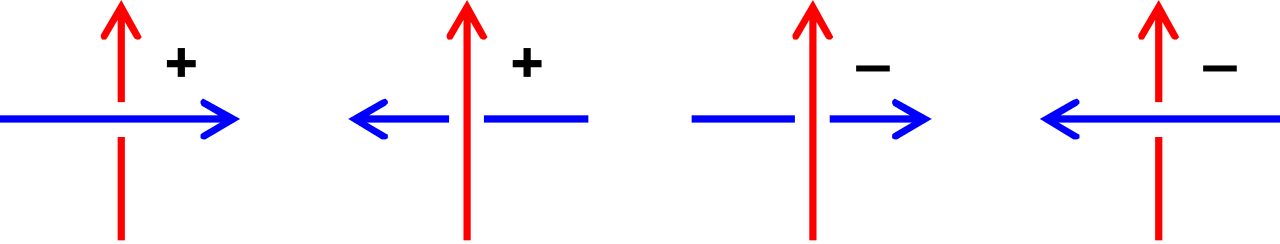
\includegraphics[width=.4\textwidth]{Pictures/Link_Crossings}}
  		
		\item Denoting as $n1, n2, n3, n4$ the number of crossings of each of the four types.
			$${\displaystyle {\text{linking number}}={\frac {n_{1}+n_{2}-n_{3}-n_{4}}{2}}}$$
	\end{itemize}
	\centering Examples
	\begin{columns}
		\begin{column}{.33\linewidth}	
			\centering{	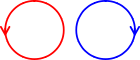
\includegraphics[width=.8\textwidth]{Pictures/UnknotsGauss}}
		\end{column}
		\begin{column}{.33\linewidth}
			\centering{	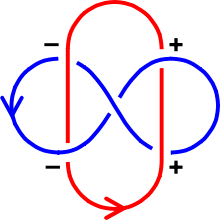
\includegraphics[width=.8\textwidth]{Pictures/WhiteheadGauss}}
		\end{column}
		\begin{column}{.33\linewidth}
			\centering{	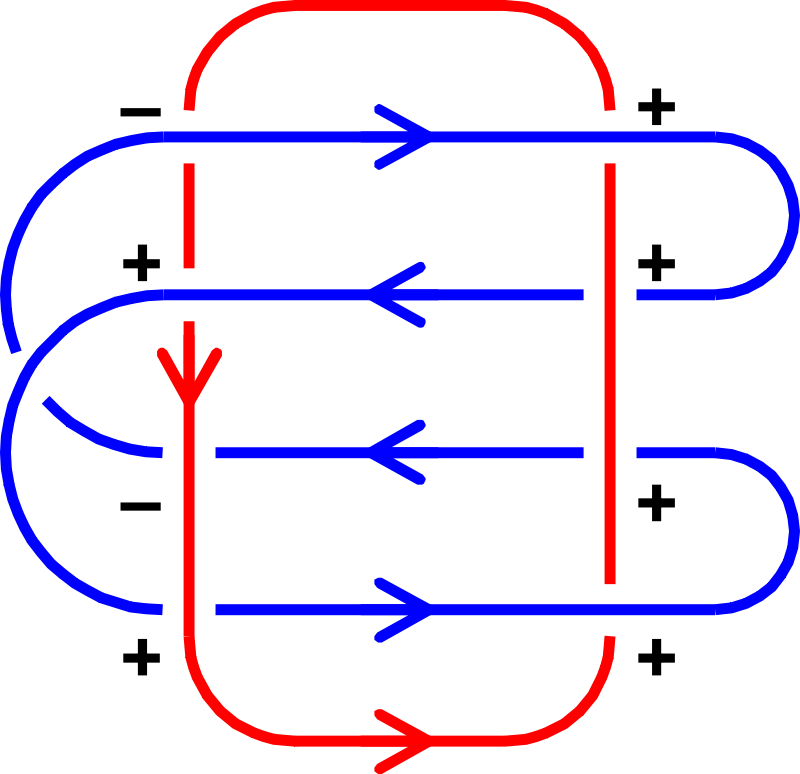
\includegraphics[width=.8\textwidth]{Pictures/Linking_Number_Example}}
		\end{column}
	\end{columns}

	
\end{frame}
\note[itemize]{
	\item \underline{recall:}
		Linking number is a numerical invariant that describes the linking of two closed curves in three-dimensional space. 
		Intuitively, the linking number represents the number of times that each curve winds around the other.
	\item 	 
		The linking number is always an integer, but may be positive or negative depending on the orientation of the two curves.
	\item
		Reversing the orientation of either of the curves negates the linking number, while reversing the orientation of both curves leaves it unchanged.
	\item See \url{https://en.wikipedia.org/wiki/Linking_number}
}
%------------------------------------------------------------------------------------------------

\end{document}